\documentclass{article}

% if you need to pass options to natbib, use, e.g.:
\PassOptionsToPackage{numbers, compress}{natbib}
% before loading neurips_2026

% The authors should use one of these tracks.
% Before accepting by the NeurIPS conference, select one of the options below.
% 0. "default" for submission
\usepackage[dblblindworkshop]{neurips_2026}
% the "default" option is equal to the "main" option, which is used for the Main Track with double-blind reviewing.
% 1. "main" option is used for the Main Track
%  \usepackage[main]{neurips_2026}
% 2. "position" option is used for the Position Paper Track
%  \usepackage[position]{neurips_2026}
% 3. "eandd" option is used for the Evaluations & Datasets Track
 % \usepackage[eandd]{neurips_2026}
% 4. "creativeai" option is used for the Creative AI Track
%  \usepackage[creativeai]{neurips_2026}
% 5. "sglblindworkshop" option is used for the Workshop with single-blind reviewing
 % \usepackage[sglblindworkshop]{neurips_2026}
% 6. "dblblindworkshop" option is used for the Workshop with double-blind reviewing
%  \usepackage[dblblindworkshop]{neurips_2026}
% 7. "education" option is used for the Education Track
%  \usepackage[education]{neurips_2026}


% After being accepted, the authors should add "final" behind the track to compile a camera-ready version.
% 1. Main Track
 % \usepackage[main, final]{neurips_2026}
% 2. Position Paper Track
%  \usepackage[position, final]{neurips_2026}
% 3. Evaluations & Datasets Track
 % \usepackage[eandd, final]{neurips_2026}
% 4. Creative AI Track
%  \usepackage[creativeai, final]{neurips_2026}
% 5. Workshop with single-blind reviewing
%  \usepackage[sglblindworkshop, final]{neurips_2026}
% 6. Workshop with double-blind reviewing
%  \usepackage[dblblindworkshop, final]{neurips_2026}
% Note. For the workshop paper template, both \title{} and \workshoptitle{} are required, with the former indicating the paper title shown in the title and the latter indicating the workshop title displayed in the footnote.
% For workshops (5., 6.), the authors should add the name of the workshop, "\workshoptitle" command is used to set the workshop title.
% \workshoptitle{WORKSHOP TITLE}
% 7. Education Track
% \usepackage[education, final]{neurips_2026}

% "preprint" option is used for arXiv or other preprint submissions
 % \usepackage[preprint]{neurips_2026}

% to avoid loading the natbib package, add option nonatbib:
%    \usepackage[nonatbib]{neurips_2026}

\usepackage[utf8]{inputenc} % allow utf-8 input
\usepackage[T1]{fontenc}    % use 8-bit T1 fonts
\usepackage{hyperref}       % hyperlinks
\usepackage{url}            % simple URL typesetting
\usepackage{booktabs}       % professional-quality tables
\usepackage{amsfonts}       % blackboard math symbols
\usepackage{nicefrac}       % compact symbols for 1/2, etc.
\usepackage{microtype}      % microtypography
\usepackage{xcolor}         % colors
\usepackage{natbib}
\usepackage{tikz}
\usepackage{verbatim}
\usepackage{fancyvrb}
\usepackage{subcaption}
\usepackage{amssymb}
\usepackage{amsmath}
\usepackage{bbm}
\usepackage{enumitem}
\usetikzlibrary{arrows.meta,calc,positioning}

\setlength{\textfloatsep}{8pt plus 2pt minus 2pt}
\setlength{\floatsep}{8pt plus 2pt minus 2pt}
\setlength{\intextsep}{8pt plus 2pt minus 2pt}
\setlength{\abovecaptionskip}{4pt}
\setlength{\belowcaptionskip}{-2pt}
%\setlist[itemize]{leftmargin=*, topsep=2pt, itemsep=1pt, parsep=0pt}

\input{macros}

% Note. For the workshop paper template, both \title{} and \workshoptitle{} are required, with the former indicating the paper title shown in the title and the latter indicating the workshop title displayed in the footnote. 
% \workshoptitle{The First Workshop on Interpreting Agent Behavior - NeurIPS 2026}
\title{How Agents Know but Fail to Act:\\ Belief Action Gap in Language Model Agents}


% The \author macro works with any number of authors. There are two commands
% used to separate the names and addresses of multiple authors: \And and \AND.
%
% Using \And between authors leaves it to LaTeX to determine where to break the
% lines. Using \AND forces a line break at that point. So, if LaTeX puts 3 of 4
% authors names on the first line, and the last on the second line, try using
% \AND instead of \And before the third author name.


\author{%
  David S.~Hippocampus\thanks{Use footnote for providing further information
    about author (webpage, alternative address)---\emph{not} for acknowledging
    funding agencies.} \\
  Department of Computer Science\\
  Cranberry-Lemon University\\
  Pittsburgh, PA 15213 \\
  \texttt{hippo@cs.cranberry-lemon.edu} \\
  % examples of more authors
  % \And
  % Coauthor \\
  % Affiliation \\
  % Address \\
  % \texttt{email} \\
  % \AND
  % Coauthor \\
  % Affiliation \\
  % Address \\
  % \texttt{email} \\
  % \And
  % Coauthor \\
  % Affiliation \\
  % Address \\
  % \texttt{email} \\
  % \And
  % Coauthor \\
  % Affiliation \\
  % Address \\
  % \texttt{email} \\
}


\begin{document}


\maketitle


\begin{abstract}
Incorrect actions can arise from inaccurate state beliefs, inappropriate values, or a failure to use available information. We study these possibilities in GPT-OSS-20B acting in a text-rendered DoorKey grid world, using explicit reports, activation probes, inverse reinforcement learning, and forced-action readouts. Task-relevant state and planner-optimal action information is often recoverable even when the emitted action is suboptimal, and the mean belief--action gap falls after reasoning despite higher decoded belief entropy. During reasoning, action preferences stabilise near the middle of the trace; report uncertainty falls around this point, but individual report corrections do not explain action changes. Reasoning-text interventions reliably redirect actions, whereas interventions at the reasoning-window activation readout site do not outperform their controls, separating decodability from causal control.
\end{abstract}


\section{Introduction}

The same wrong action can have different causes. An agent may misread its environment, assign the wrong value to a correctly represented state, or fail to use available information when selecting an action. Output accuracy alone does not distinguish these cases, although they call for different explanations and interventions.

We separate three components of a decision. A \emph{belief} is an interpretable representation of the current environment state. A \emph{value} ranks possible states or their consequences. \emph{Action selection} maps the available beliefs and values to an emitted action. A belief--action gap occurs when the emitted action is worse than an available alternative under the model's estimated belief and inferred value function.

Activation probes can identify encoded spatial information \cite{li2023emergent,nanda-etal-2023-emergent,gurnee2024language,arghal2026behavioural}, and inverse reinforcement learning can recover preferences from behaviour \cite{ng2000algorithms,ziebartMaximumEntropyInverse2008a}. Separate work studies when answers become decodable during reasoning and whether chain-of-thought text reflects the computation that produced an answer \cite{pal-etal-2023-future,dong2025emergent,lanham2023measuring}. The missing link is a joint account of what information is available, when an action forms, and which measured state can causally control it.

We study GPT-OSS-20B in a fully observable DoorKey task with known dynamics and shortest-path actions. Our contributions are: (1) a diagnostic that combines report and activation-based beliefs with learned values to separate state errors from downstream action mismatch; (2) a temporal analysis showing how forced-action preferences stabilise during reasoning; and (3) causal tests comparing reasoning-text interventions with interventions on the reasoning-window activation state. The results support one sequence: task information is available, action preferences form during reasoning, and causal control is stronger through the generated text than through the activation readout site we tested.


\section{Measurement Framework}
\label{sec:estimating}

We describe a decision by an estimated belief $\hat q_{t,p}(s)$ over the current state, a learned state-value function $g_\theta(s)$, and the emitted action $a_t$. Values rank successor states; action selection is the process that produces $a_t$ from the information available to the model. The belief--action gap measures whether $a_t$ is consistent with the best action under the estimated belief and learned values.

\begin{figure}[t]
\centering
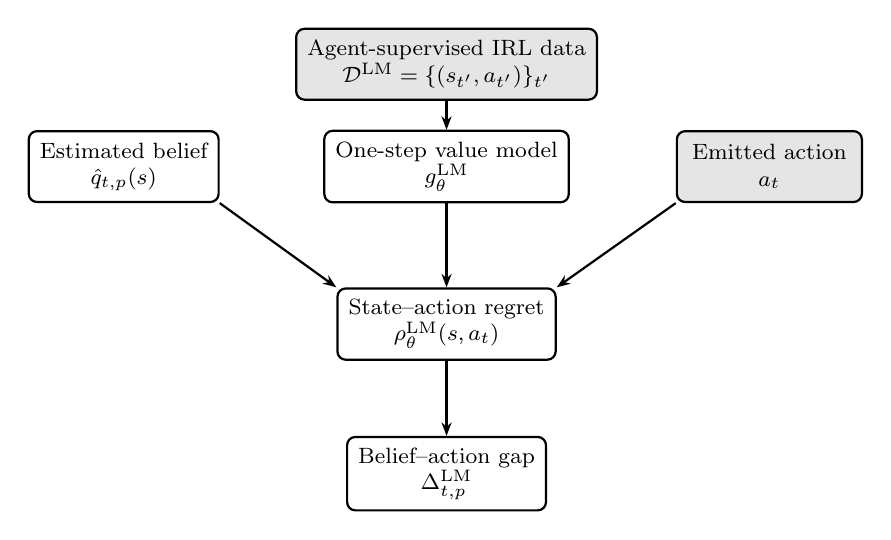
\begin{tikzpicture}[
 every node/.style={font=\footnotesize,align=center},
 box/.style={rounded corners=3pt,draw=black,thick,minimum height=0.9cm,minimum width=2.35cm,inner sep=4pt},
 observable/.style={box,fill=black!10},
 arrow/.style={-{Stealth[length=1.7mm]},thick}]
\node[observable, minimum width=3.0cm] (data) at (4.1,1.3) {Agent-supervised IRL data\\$\mathcal D^{\mathrm{LM}}=\{(s_{t'},a_{t'})\}_{t'}$};
\node[box] (belief) at (0,0) {Estimated belief\\$\hat q_{t,p}(s)$};
\node[box] (value) at (4.1,0) {One-step value model\\$g_\theta^{\mathrm{LM}}$};
\node[observable] (action) at (8.2,0) {Emitted action\\$a_t$};
\node[box] (regret) at (4.1,-2.0) {State--action regret\\$\rho_\theta^{\mathrm{LM}}(s,a_t)$};
\node[box] (gap) at (4.1,-3.9) {Belief--action gap\\$\Delta_{t,p}^{\mathrm{LM}}$};
\draw[arrow] (data.south) -- (value.north);
\draw[arrow] (belief.south east) -- (regret.north west);
\draw[arrow] (value.south) -- (regret.north);
\draw[arrow] (action.south west) -- (regret.north east);
\draw[arrow] (regret.south) -- (gap.north);
\end{tikzpicture}
\caption{Operational decomposition. Grey boxes are observed. Estimated beliefs, the learned value model, and the emitted action determine the belief--action gap.}
\label{fig:belief_action_pipeline}
\end{figure}

\subsection{Environment and Data}
\label{sec:env-data}

The main experiments use a fully observable, text-rendered DoorKey grid world \cite{arghal2026behavioural}. A state is $s_t=(x_t,y_t,h_t,d_t)$: agent coordinates, key possession, and door status. The model sees the current grid and key status, but no earlier environment states or actions, then emits one of $\{\textsc{left},\textsc{right},\textsc{up},\textsc{down}\}$. Transitions are deterministic: a valid move changes position by one cell, while a wall or locked door leaves the state unchanged. We use A$^\star$ on this state space to define $A_G^*(s)$, the set of actions whose successor lies on a shortest valid path to the goal. The endpoint analyses use a fixed $9\times9$ layout with 39 walkable cells and 117 reachable task states. Other cohorts use the same DoorKey task unless marked as a matched local-wall control.

\begin{figure}[htbp]
\centering
\begin{subfigure}[c]{0.42\textwidth}
\centering
\begin{BVerbatim}
  0 1 2 3 4 5 6 7 8
0 # # # # # # # # #
1 # . . . # . . . #
2 # . . . D . . . #
3 # . . . # . G . #
4 # . # # # # # # #
5 # . . . . . . . #
6 # . . . # . K . #
7 # . . A # . . . #
8 # # # # # # # # #
\end{BVerbatim}
\caption{}\label{fig:grid_text}
\end{subfigure}\hspace{0.02\textwidth}
\begin{subfigure}[c]{0.42\textwidth}
\centering
\includegraphics[width=0.6\linewidth]{figures/keydoorenv.png}
\caption{}\label{fig:grid_visual}
\end{subfigure}
\caption{A DoorKey state in the model's text input and as a spatial rendering. $A$, $K$, $D$, and $G$ denote the agent, key, door, and goal.}
\label{fig:environment}
\end{figure}

\begin{table}[t]
\centering\small
\begin{tabular}{p{0.25\linewidth}p{0.26\linewidth}p{0.39\linewidth}}
\toprule
Cohort & Coverage & Analyses \\
\midrule
Endpoint state and gap & 200 trajectories; 3,194 decisions; fixed $9\times9$ DoorKey layout & State probes and pre/post belief--action gap \\
IRL & 100 trajectories; 1,822 transitions; fixed $9\times9$ DoorKey layout & Agent-supervised and planner-supervised value models \\
Report probes & 33 failure cases; focused slice of 13 decisions & Directional state reports and three wall-hit contradictions \\
Reasoning corpus & 95 DoorKey trajectory files; 1,276 decisions & 98,310 forced-action prefixes and commitment timing \\
Matched reasoning cohort & 31 trajectories; 46 decisions & Beliefs, attention, activations, and action-revision controls \\
Matched local-wall control & 15 states; $7\times7$ grid slice & Report and layer-15 wall readouts on the same state--direction pairs \\
Text interventions & 396 mismatched plus 396 congruent pairs; 240 injection cuts & Whole-chain replacement and sentence injection \\
\bottomrule
\end{tabular}
\caption{Datasets used in the reported analyses. Cohorts are separate unless stated otherwise.}
\label{tab:data-summary}
\end{table}

\subsection{Belief and Value Estimates}
\label{sec:estimating-beliefs}

\paragraph{Representation probes.}\label{sec:activation-based-estimation}
We fit linear probes to GPT-OSS-20B activations to predict agent location, key possession, and door status. Separate probes are evaluated immediately before reasoning and immediately before the answer. Their categorical outputs are combined and normalised over valid DoorKey states to obtain $q_{t,p}^{\mathrm{probe}}(s)$. Decodability establishes information availability, not causal use. Architecture, preprocessing, and split details are in \Cref{app:representation-probes}.

\paragraph{Report probes.}
We separately ask the model categorical and coordinate questions about the rendered state and one-step action consequences. These forward passes measure what the model can explicitly report; they are not activations from the original action-generation pass. Prompt templates, answer categories, parsing, and the panels used in each analysis are in \Cref{app:report-protocol}.

\paragraph{Inverse reinforcement learning.}\label{sec:estimating-values}
We learn a linear value $g_\theta$ over activation-derived state representations. A one-step Boltzmann policy scores each action by the value of its deterministic successor. We fit one model to the LM's emitted actions and another to planner-optimal actions, using state-disjoint training and validation splits. Optimisation, feature construction, and missing-state handling are in \Cref{app:irl-details}.

\subsection{Belief--Action Gap}\label{sec:belief-action-gap}
For diagnosis only, without claiming that the model performs this calculation, we define action utility as
\begin{align}
U_{\theta,t,p}(a)=\mathbb{E}_{s\sim \hat q_{t,p}}\!\left[g_\theta(T_G(s,a))\right].
\label{eq:expected-action-preference}
\end{align}
The belief--action gap is the utility lost by the emitted action:
\begin{align}
\Delta_{t,p}^{\mathrm{LM}}=\max_{a\in\mathcal A}U_{\theta,t,p}(a)-U_{\theta,t,p}(a_t).
\label{eq:belief-action-gap}
\end{align}
A large gap means that another action has higher inferred utility under the decoded belief. This separates inaccurate state estimates from downstream mismatch between available state information, inferred preferences, and the emitted action.


\section{Information Availability and Action Mismatch}
\label{sec:analysis1}

Task-relevant state and planner-optimal action structure are recoverable from model activations, but the model's realised actions are less predictable. Explicit reports provide direct cases in which the model states the relevant fact and acts against it.

\subsection{State Information}\label{sec:belief-results}
On state-disjoint held-out decisions, key possession and door status are decoded reliably, while exact location is harder (\Cref{tab:rep-beliefs}). Uniform top-1 accuracy over the 39 valid locations is 2.56\%. The probe is above this baseline before and after reasoning, although every state metric declines at the later readout.

\begin{table}[htbp]
\centering\small
\begin{tabular}{lcc}
\toprule
Metric & Before reasoning & After reasoning \\
\midrule
Key possession accuracy & 100.0\% & 89.5\% \\
Door status accuracy & 100.0\% & 88.6\% \\
Location top-1 accuracy & 34.8\% & 13.1\% \\
Top-1 within Manhattan distance 1 & 95.5\% & 60.8\% \\
Top-1 within Manhattan distance 2 & 99.0\% & 83.5\% \\
Probability mass within distance 1 & 93.1\% & 59.2\% \\
Probability mass within distance 2 & 97.2\% & 81.5\% \\
\bottomrule
\end{tabular}
\caption{Representation-based state decoding on held-out decision states. Top-1 distance uses the most probable decoded location; probability mass sums over all locations within the stated Manhattan distance.}
\label{tab:rep-beliefs}
\end{table}

Reports and activation probes can also be compared on the same local questions. The matched control contains 15 states and four directions per state. It has 8 wall, 49 empty, and 3 goal neighbours; no adjacent key or door occurs. Reports identify all 60 cases correctly, while the layer-15 activation probe is weakest on walls (\Cref{tab:matched-wall}).

\begin{table}[htbp]
\centering\small
\begin{tabular}{lrrr}
\toprule
True adjacent cell & $n$ & Report & Probe before / after \\
\midrule
Wall & 8 & 100.0\% & 25.0\% / 50.0\% \\
Empty & 49 & 100.0\% & 93.9\% / 93.9\% \\
Goal & 3 & 100.0\% & 100.0\% / 100.0\% \\
\bottomrule
\end{tabular}
\caption{Matched accuracy for the question ``Is the adjacent cell a wall?'', grouped by the true cell rather than direction. Counts are state--direction pairs.}
\label{tab:matched-wall}
\end{table}

The clearest behavioural contradiction occurs in a prespecified 13-decision failure slice. It contains three wall-hit decisions, defined as emitted moves into blocked neighbouring cells. At 0, 25, 50, 75, and 100\% of the original reasoning, with the final action hidden, the model reports the chosen direction as blocked in all three cases and still originally chose that move. Full report accuracy and selection details are in \Cref{app:report-protocol}.

\subsection{Action-Value Structure}\label{sec:value-results}
The planner-supervised value model predicts shortest-path actions almost perfectly, while the agent-supervised model predicts only about 59\% of emitted actions (\Cref{tab:value-results}). Thus, the activation-derived state representations support task-optimal action structure more reliably than the model's realised policy.

\begin{table}[htbp]
\centering\small
\begin{tabular}{lcc}
\toprule
Value model & Before reasoning & After reasoning \\
\midrule
Agent-supervised & 58.8\% & 59.0\% \\
Planner-supervised & 99.7\% & 99.5\% \\
\bottomrule
\end{tabular}
\caption{Held-out action accuracy of one-step value models using activation-derived state representations.}
\label{tab:value-results}
\end{table}

\subsection{Belief--Action Gap}\label{sec:decomposition}
We evaluate the gap on 3,194 decisions from 200 trajectories; the value model is fitted on the separate 100-trajectory cohort. The mean gap falls after reasoning in the full data, among the 2,465 decisions for which every state probe is correct, and on held-out probe states (\Cref{tab:gap-pre-post}). Decoded belief entropy rises in all three comparisons. The emitted action therefore becomes more consistent with the inferred subjective value function without a sharper decoded state estimate.

\begin{table}[htbp]
\centering\small
\begin{tabular}{lccccc}
\toprule
Subset & $n$ & $\Delta_{\mathrm{before}}$ & $\Delta_{\mathrm{after}}$ & $H_{\mathrm{before}}$ & $H_{\mathrm{after}}$ \\
\midrule
All decisions & 3,194 & 0.955 & 0.583 & 1.494 & 2.085 \\
All probes correct & 2,465 & 0.908 & 0.558 & 1.106 & 1.811 \\
Probe held-out states & 762 & 1.106 & 0.665 & 2.788 & 3.020 \\
\bottomrule
\end{tabular}
\caption{Mean belief--action gap $\Delta$ and decoded belief entropy $H$ before and after reasoning.}
\label{tab:gap-pre-post}
\end{table}

Together, these results locate a mismatch downstream of information availability: relevant state facts and task-optimal action structure can be recovered, yet they do not always govern the emitted action. Additional value controls and examples are in \Cref{app:value-controls}.


\section{How Actions Stabilise During Reasoning}\label{sec:reasoning}
The reasoning corpus contains 95 DoorKey trajectory files, 1,276 decisions, and 2,370,850 reasoning tokens. We evaluate 98,310 prefixes, at most 80 per decision. Sentence segmentation and prefix sampling are described in \Cref{app:reasoning-measurement}.

\subsection{Action Preference and Commitment}\label{sec:commitment}
At each prefix $p$, we append a fixed answer suffix and normalise the logits of the four action tokens to obtain $\pi_{t,p}(a)$ (\Cref{app:answer-forcing}). The preferred action is $\arg\max_a\pi_{t,p}(a)$. Commitment is the first evaluated prefix that begins the final segment over which this preferred action never changes.

The probability assigned to the eventually emitted action and the inverse normalised entropy both rise during reasoning (\Cref{fig:commitment-measures}). The median commitment position is 0.49 of the reasoning tokens, leaving a median 50.6\% of the trace, or 524 tokens, after commitment. A smaller matched check finds later commitment in 23 failure decisions than in 23 controls, at 130 versus 97 sentences on average; the uncertainty intervals overlap, so this difference is descriptive. Alternative timing definitions, action-mention controls, and switch rates are in \Cref{app:alternative-commitment}.

\begin{figure}[t]
\centering
\includegraphics[width=\textwidth]{figures/commitment_measures_panel_v2.png}
\caption{Action preference over 98,310 prefixes from 1,276 decisions. Left: mean probability of the emitted action and inverse normalised entropy over reasoning progress, including the subset before the first decisional action mention. Right: probability of the emitted action by action class. Bands are 95\% intervals obtained by resampling complete trajectories.}
\label{fig:commitment-measures}
\end{figure}

\subsection{What Changes Around Commitment}\label{sec:belief-commitment}
The matched reasoning analysis contains 46 decisions from 31 trajectories, 7,084 sentence prefixes, and 42,504 reports about four adjacent walls, key possession, and door status. The paired comparison uses 45 decisions from 30 trajectories with reports both before and at or after commitment. Report entropy falls by 0.056 bits, while accuracy changes by only 0.2 percentage points (\Cref{tab:belief-commitment-changes}).

\begin{table}[t]
\centering\small
\begin{tabular}{lrrr}
\toprule
Measure & Before & At or after & Change [95\% interval] \\
\midrule
Belief entropy (bits) & 0.392 & 0.336 & $-0.056\;[-0.105,-0.009]$ \\
Report accuracy & 82.8\% & 83.0\% & $+0.2\;[0.0,0.6]$ pp \\
\bottomrule
\end{tabular}
\caption{Reported beliefs around retrospective commitment. Values are averaged within decisions and then across decisions. Intervals are obtained by resampling complete trajectories.}
\label{tab:belief-commitment-changes}
\end{table}

Report corrections rarely coincide exactly with action changes: at least one of six reports changes correctness at 14 of 682 action changes (2.1\%), 6 of 161 optimal-to-suboptimal changes (3.7\%), and 3 of 182 suboptimal-to-optimal changes (1.6\%). The full transition results and the attention, change-point, semantic, and activation analyses are in \Cref{app:action-revision-correlates,app:semantic-clustering}. These analyses identify correlates of action formation but not its cause.


\section{What Causally Controls the Action}\label{sec:causal}
Reasoning-text interventions redirect actions, whereas activation interventions at the reasoning-window readout site do not outperform their controls. We use sentence boundaries because report and action changes are measured there. We edit the final reasoning-window residual state because commitment is strongly decodable at that site; this tests causal use at the readout location, not at pre-reasoning activations.

\subsection{Reasoning-Text Interventions}\label{sec:text-patching}\label{sec:targets}
Whole-chain replacement pairs one decision's prompt with reasoning from a decision that ends in another action. Across 396 mismatched pairs and 396 congruent controls, the forced action follows the foreign reasoning at early, middle, and late cuts; full results are in \Cref{app:intervention-robustness}.

For a local test, we sample 240 prefix cuts and append counter-evidence naming the current runner-up action, a neutral sentence, or support for the current top action. Among 201 cases where the injected action differs from the eventual action, counter-evidence changes the forced top action to the injected action in all 81 cuts below commitment 0.7, 92.5\% at 0.7--0.85, 90.0\% at 0.85--0.95, and 62.5\% at or above 0.95 (\Cref{fig:injection}). The decline with commitment is significant ($\rho=-0.421$, $p=5.0\times10^{-10}$), but commitment also covaries with reasoning progress. Neutral text changes the top action in 9.6\% of cuts.

\begin{figure}[t]
\centering
\includegraphics[width=\textwidth]{figures/commitment_gated_injection.png}
\caption{Single-sentence intervention at 240 prefix cuts. Left: rate at which the forced action follows counter-evidence or neutral text, grouped by the probability assigned to the eventual action before injection. Right: mean change in probability assigned to the named action. Bars are Wilson 95\% intervals.}
\label{fig:injection}
\end{figure}

\subsection{Activation Interventions}\label{sec:activation-patching}
We intervene on residual activations of the final reasoning-window tokens. Steering along a decoded action or commitment direction changes 13.5\% of answers to the intended action at the largest magnitude tested, compared with 13.0\% for a norm-matched random direction (Fisher's exact $p=1.00$). Replacing the entire $12\times2{,}880$ window state with a donor state changes 20.8\% of answers to the donor action at the strongest layer tested; smaller rank-1 and rank-3 transplants change none. Thus, the tested activation edits do not provide targeted control beyond their controls. Layer sweeps, deletion, instruction controls, and limitations are in \Cref{app:intervention-robustness}.

\begin{figure}[t]
\centering
\includegraphics[width=0.9\textwidth]{figures/readwrite_asymmetry.png}
\caption{Commitment is decodable from the reasoning-window activation state, but steering does not outperform a norm-matched random direction. The full intervention comparison is reported in \Cref{app:intervention-robustness}.}
\label{fig:readwrite}
\end{figure}

\paragraph{Synthesis.}
The probe and IRL results establish availability: state and task-optimal action information can be recovered. Prefix readouts establish formation: action preferences sharpen and reach a final stable segment during reasoning. Only the intervention results test causal use. They show that generated reasoning text can redirect the action, while the reasoning-window activation state is readable but was not a reliable control point under the interventions tested.


\section{Discussion}\label{sec:discussion}
The results separate information availability from action formation and causal use. State variables and planner-optimal action structure are recoverable, but this information does not always determine behaviour. The three wall-hit cases make the mismatch concrete: the model reports the obstacle and still selects the blocked action.

Reasoning narrows the mismatch without simply sharpening the decoded state. The belief--action gap falls after reasoning while decoded state entropy rises. Prefix readouts then show when action preferences stabilise, and reports become less uncertain around that point. The weak alignment between report corrections and action changes argues against a simple account in which commitment is caused by fixing one local state belief.

The causal tests distinguish two intervention sites. Short changes to the generated reasoning often redirect the forced action, even late in the trace. By contrast, activation steering at a site where commitment is easy to decode does not beat a norm-matched random control. This negative result is limited to the layers, directions, magnitudes, and window tested; it does not show that activations are causally irrelevant in general.

The study is limited to GPT-OSS-20B in controlled DoorKey tasks. Beliefs and values are operational estimates, the value model is one-step, and commitment is defined retrospectively over sampled prefixes. These choices make the failure modes measurable, but broader environments and models are needed to test generality.

\section{Conclusion}\label{sec:conclusion}
A model can contain task-relevant information without using it reliably. In DoorKey, state and planner-optimal action information are recoverable before the emitted action, action preferences stabilise during reasoning, and the belief--action gap falls even as decoded state uncertainty rises. Text interventions redirect decisions, while interventions on the reasoning-window activation readout site do not outperform their controls. Availability, formation, and causal use are therefore distinct claims and require distinct tests.


% \begin{ack}
% Use unnumbered first level headings for the acknowledgments. All acknowledgments
% go at the end of the paper before the list of references. Moreover, you are required to declare
% funding (financial activities supporting the submitted work) and competing interests (related financial activities outside the submitted work).
% More information about this disclosure can be found at: \url{https://neurips.cc/Conferences/2026/PaperInformation/FundingDisclosure}.


% Do {\bf not} include this section in the anonymized submission, only in the final paper. You can use the \texttt{ack} environment provided in the style file to automatically hide this section in the anonymized submission.
% \end{ack}

%\section*{References}

\bibliography{ref}
\bibliographystyle{abbrvnat}



%%%%%%%%%%%%%%%%%%%%%%%%%%%%%%%%%%%%%%%%%%%%%%%%%%%%%%%%%%%%

\appendix

\section{Measurement Details}

\subsection{Representation Probes}\label{app:representation-probes}
The endpoint probes use the 200-trajectory cohort and split by environment state: all occurrences of a state are assigned to either the 80\% training set or the 20\% held-out set. Before reasoning, the input is the concatenation of the last three prompt-token activations; after reasoning, it is the last three reasoning-token activations. Each token vector has 2,880 dimensions, giving an 8,640-dimensional input. Separate L2-regularised logistic regressions predict location, key possession, and door status after feature-wise standardisation fitted on the training split. Location is one categorical variable over valid cells. The three output distributions are multiplied and renormalised over the 117 valid task states. We evaluate layers 7, 15, and 23 with the same specification rather than choosing a separate model for each condition.

\subsection{Inverse Reinforcement Learning}\label{app:irl-details}
For each covered state, we average its activation-derived representations across occurrences. The linear value model scores each deterministic successor representation, and a softmax over the four scores defines the one-step policy. We train separate models on emitted actions and planner-optimal actions using a state-disjoint split. Training uses Adam for 500 epochs, initial learning rate $10^{-3}$, cosine annealing, gradient clipping at 1.0, fixed inverse temperature $\beta=1$, and L2 regularisation; the selected checkpoint maximises held-out log-likelihood. If any of a source state's four successors lacks an activation-derived representation, that source state is excluded rather than imputed.
\subsection{Report-Based Probe Protocol}
\label{app:report-protocol}

For report-based belief estimation, we use a total of 38 questions: 30 categorical questions and eight coordinate questions.
Every prompt begins by describing the fully observable $9\times9$ DoorKey environment, giving the symbol legend, and defining \textsc{right}, \textsc{left}, \textsc{up}, and \textsc{down} as cardinal directions in the rendered grid.
It then supplies the current grid.
Endpoint prompts include the carrying-key status for questions configured to require it; reasoning-time prompts include this status and the reasoning prefix $R_{t,\leq p}$.

\paragraph{Categorical question templates.}
The 30 categorical questions are generated from the following templates, where $d\in\{\textsc{right},\textsc{left},\textsc{up},\textsc{down}\}$, $a$ ranges over the corresponding four moves, and $o\in\{\text{goal},\text{key},\text{door}\}$:
\begin{enumerate}
    \item ``Given the current grid only, do you currently have the key?'' and ``Given the current grid only, is any door currently open?'' (two questions);
    \item ``Given the current grid only, is the cell immediately $d$ of the agent a wall (\texttt{\#})?'' (four questions);
    \item ``Given the current grid only, is the $o$ immediately to your $d$?'' (12 questions);
    \item ``Given the current grid only, if you move $a$ now, will you hit a wall?'', ``will you have the key after that move?'', and ``will the grid still show an open door (\texttt{O}) after that move?'' (12 questions).
\end{enumerate}
The requested output is exactly one label: \texttt{A=yes}, \texttt{B=no}, or \texttt{C=unknown}.

\paragraph{Coordinate question templates.}
Four questions ask for the current location of the agent, goal, key, or a door, and four ask for the agent's location after each candidate move.
The requested output is exactly \texttt{\{"row": <int>, "col": <int>\}}.
For a current object that is not visible, the prompt specifies $(-1,-1)$; rows and columns are zero-indexed grid coordinates.

\paragraph{Post-processing and scores.}
Categorical text is lower-cased and stripped of surrounding quotation marks and terminal punctuation.
Only an exact \texttt{A}/\texttt{B}/\texttt{C} or \texttt{yes}/\texttt{no}/\texttt{unknown} is accepted; other text is \texttt{invalid} rather than being matched fuzzily.
For repeated generations, every sample, including \texttt{invalid}, contributes to the empirical distribution.
For API log-probability runs, we exponentiate and renormalise the recognised \texttt{A}/\texttt{B}/\texttt{C} mass at the answer-token position and record missing candidates and excluded top-$k$ mass.
For the local scaled run, we score all three candidate tokens directly at the final answer position, divide the logits by temperature $0.7$, and apply softmax.

For coordinate responses, we extract a JSON object and accept it only when both \texttt{row} and \texttt{col} are integers.
Repeated coordinate samples are summarised by their modal valid coordinate; we additionally record parse rate, the number of distinct coordinates, and mean Manhattan error.

\paragraph{Panels used.}
The reasoning-time panel uses \texttt{wall\_left/right/up/down}, \texttt{has\_key}, and \texttt{door\_open}, plus \texttt{hit\_wall\_after\_$a$}, \texttt{has\_key\_after\_$a$}, and \texttt{door\_open\_after\_$a$} for the action read out at that position.
Earlier small-scale reasoning runs additionally query \texttt{agent\_location}, \texttt{goal\_location}, \texttt{key\_location}, and \texttt{door\_location}; the scaled matched-cohort run defers these coordinate questions.
Other endpoint analyses select question families from the same 38-question registry.

\begin{table}[htbp]
\centering
\small
\begin{tabular}{lccc}
\toprule
Query family & State--question pairs & Greedy & Ten-sample modal \tabularnewline
\midrule
Wall & 132 & 93.9\% & 97.0\% \tabularnewline
Goal adjacency & 132 & 100.0\% & 100.0\% \tabularnewline
Door adjacency & 132 & 99.2\% & 100.0\% \tabularnewline
Key adjacency & 132 & 67.4\% & 97.0\% \tabularnewline
\bottomrule
\end{tabular}
\caption{Report accuracy on the 33-state failure-mode set. Each family contains four directional questions per state. The modal result uses ten samples per question at temperature 0.7.}
\label{tab:report-accuracy-33}
\end{table}

\subsection{Answer Forcing}
\label{app:answer-forcing}
For the prefix-level action distributions of \Cref{sec:commitment} (98,310 prefixes), we truncate the reasoning trace at the prefix and append a fixed 12-token suffix that closes the reasoning channel and opens the final-answer JSON in the model's chat format:
\begin{quote}
\ttfamily
<|end|><|start|>assistant<|channel|>final<|message|>\{\par
\ \ "action": "
\end{quote}
The token sequence of the suffix is checked against the tokenizer at load time.
We read the logits of the four single-token candidates \texttt{UP}, \texttt{DOWN}, \texttt{LEFT}, and \texttt{RIGHT} at the next position and normalise them with a softmax; no natural-language instruction is added, and every prefix is scored with an independent forward pass without reuse of cached model state.

\subsection{Reasoning Corpus and Sentence Segmentation}\label{app:reasoning-measurement}
The source is the 95 files present in the nominal 100-trajectory DoorKey corpus. We remove the terminal action JSON, then segment each reasoning trace as follows:
\begin{enumerate}
\item Mark blank lines and sentence-ending punctuation followed by whitespace as candidate boundaries.
\item Do not split after a decimal point, a recognised abbreviation, a coordinate component, or the period in a numbered action.
\item Keep any embedded action JSON as one span.
\item If a resulting fragment contains fewer than ten characters, join it to an adjacent fragment.
\end{enumerate}
The chunker records each unit's character offsets. GPT-OSS-20B token offsets are intersected with those spans to record token boundaries. This produces 153,622 sentence units independently of the action-readout positions. Prefix sampling evaluates at most 80 positions per decision, with a median separation of 20 tokens and wider spacing for longer traces, producing 98,310 prefixes.

\section{Additional Value Analyses}\label{app:value-controls}
\paragraph{FourRooms label control.}
A separate FourRooms control uses identical activations and training procedures while changing only the supervision labels. Test accuracy rises from 45.4\% with agent actions to 96.0\% with A$^\star$-optimal labels; set-membership accuracy rises from 36.9\% to 99.2\%. This auxiliary environment is not part of the DoorKey main analysis.

\paragraph{Value landscape example.}
The one-step objective identifies relative preferences among available successors, so absolute values and signs should not be read as distances to the goal.
\begin{figure}[htbp]
\centering
\includegraphics[width=0.8\textwidth]{figures/traj196_step5_pre_value_compare.pdf}
\caption{Learned state values for planner-supervised IRL (left) and agent-supervised IRL (right) in one task phase. The main quantitative comparison is action ordering in \Cref{tab:value-results}.}\label{fig:irl_value_app}
\end{figure}

\paragraph{Belief--action gap example.}
\begin{figure}[htbp]
\centering
\includegraphics[width=0.8\textwidth]{figures/traj192_step5.pdf}
\caption{One decision before and after reasoning. Cell labels are decoded location probabilities. Reasoning increases entropy from 0.261 to 1.572 while reducing the gap from 2.386 to 0.205.}\label{fig:belief_viz_app}
\end{figure}

\section{Alternative Commitment Measures}\label{app:alternative-commitment}
The median first decisional action mention occurs at progress 0.30, the final stable action begins at 0.49, and the probability assigned to the emitted action permanently exceeds 0.8 at 0.65. Only 37.0\% of decisions commit before the first decisional mention. Preference switching declines from 0.133 in the first progress decile to 0.019 in the last, and 8.9\% of prefixes with emitted-action probability above 0.9 are followed by a later switch.

\begin{figure}[t]
\centering
\begin{subfigure}[b]{0.42\textwidth}
\centering\includegraphics[width=\linewidth]{figures/clocks_v2.png}
\caption{Alternative timing definitions.}\label{fig:three-clocks}
\end{subfigure}\hfill
\begin{subfigure}[b]{0.56\textwidth}
\centering\includegraphics[width=\linewidth]{figures/hazard.png}
\caption{Preference-switch rates.}\label{fig:switch-hazard}
\end{subfigure}
\caption{Alternative commitment measures and later-switch probability over 1,276 decisions.}\label{fig:commitment-dynamics}
\end{figure}

\paragraph{Reasoning after commitment.}
A four-class judge labels 141,377 sentences from 1,004 decisions as world-reading, solving, meta-checking, or concluding. World-reading falls from 68\% before commitment to 29\% after it, while solving rises from 25\% to 45\% and concluding from 1\% to 12\%. Relative to positions drawn from traces of similar length, the drop in world-reading and rise in solving are larger than expected ($p=0.01$); the rise in concluding is not ($p=0.20$).

\begin{figure}[t]
\centering
\includegraphics[width=\textwidth]{figures/coarse4_functions_v2.png}
\caption{Four coarse sentence functions before and after commitment. The lower panels align 400-character bins to commitment and compare them with positions drawn from traces of similar length.}\label{fig:sentence-functions}
\end{figure}

\subsection{Action-Mention Classification}
\label{app:action-mentions}
The pre-verbal control and the first-mention timing measure require the position of the first \emph{decisional} mention of an action in each reasoning trace.
We locate every occurrence of \textsc{up}, \textsc{down}, \textsc{left}, or \textsc{right} in the 1,276 traces (72,561 occurrences) at its token position and classify it with fixed rules applied in order: (i) \emph{idiom} --- ``pick up'', ``set up'', ``what's left'', ``that's right'' and similar (0.9\%); (ii) \emph{negated} --- a negation cue within two words before the word (``cannot go up'', ``instead of right'') or ``is blocked'', ``is a wall'', ``is not possible'' within three words after it (3.3\%); (iii) \emph{answer} --- preceded by ``answer'', ``action'', ``output'', ``choose'' or similar (3.0\%); (iv) \emph{movement} --- preceded by a movement verb such as ``go'', ``move'', ``head'', ``step'' (18.3\%); (v) \emph{capitalised} direction words (6.4\%); (vi) \emph{descriptive} --- preceded by ``to/on/at the'', ``top-'', ``bottom-'', or followed by ``side'', ``column'', ``of'', ``wall'', ``corner'' and similar (5.8\%); (vii) \emph{bare} --- all remaining occurrences, mostly route enumerations such as ``left to (1,6), left to (1,5)'' (62.2\%).
Classes (iii)--(v) and (vii) are decisional; (i), (ii) and (vi) are not.
Under the previous definition (any direction word, regardless of context) the pre-verbal subset contained 31,723 prefixes and the median first mention was at progress 0.25; under the decisional definition it contains 35,379 prefixes and the median first decisional mention is at 0.30, with 37.0\% of decisions committing before it (35.6\% under the previous definition).
Counting negated mentions as decisional changes the subset by 46 prefixes and none of the reported values.


\section{Correlates of Action Revision}\label{app:action-revision-correlates}
\label{app:additional-reasoning}

\paragraph{Report corrections at action transitions.}
\begin{table}[t]
\centering\small
\begin{tabular}{lrrr}
\toprule
Transition & Events & Any report change & $\Delta$ error [95\% interval] \\
\midrule
Any action change & 682 & 14 (2.1\%) & $0.0005\;[-0.0022,0.0027]$ \\
Optimal to suboptimal & 161 & 6 (3.7\%) & $0.0000\;[-0.0065,0.0055]$ \\
Suboptimal to optimal & 182 & 3 (1.6\%) & $-0.0018\;[-0.0080,0.0017]$ \\
\bottomrule
\end{tabular}
\caption{Changes in report correctness from the preceding sentence to an action transition. Intervals are obtained by resampling complete trajectories.}\label{tab:belief-action-transitions}
\end{table}
All six reports remain correct across 66 of 161 optimal-to-suboptimal transitions.

\paragraph{Prospective monitoring.}
Among 5,283 prefixes whose current preferred action is optimal, 347 lose optimality within three sentences. A random ranking therefore has expected AUPRC $347/5{,}283=0.066$. A model using reasoning progress, current action confidence, and change from the preceding action distribution reaches AUPRC 0.273 when evaluated on complete trajectories excluded from fitting. Adding belief reports raises AUPRC to 0.334, a difference of 0.061 with a 95\% interval $[0.014,0.123]$ obtained by resampling complete trajectories. The next-sentence result is inconclusive.

\paragraph{Attention at action changes.}
At each sentence boundary, we read attention from the final action-token query to four source regions: the newest reasoning sentence, earlier reasoning, the grid, and the key-status statement. At layer 15, averaged over all heads and source tokens in a region, the newest sentence receives 0.0838 additional percentage points of attention per token at an action change relative to a stable-action sentence from the same decision with similar reasoning progress (67 pairs; 95\% interval $[0.0442,0.1314]$). The grid, key-status statement, and earlier reasoning intervals include zero.


\paragraph{Commitment timing in matched states.}
The main analysis measures the post-commitment tail in tokens across 1,276
decisions. As a smaller matched check, we also measure commitment after each
sentence in 23 failure and 23 control decisions. Failure decisions commit after
130 sentences on average, compared with 97 for controls, and after 0.77 versus
0.68 of the reasoning characters. The intervals overlap, so this is a
descriptive difference.

\begin{figure}[htbp]
\centering
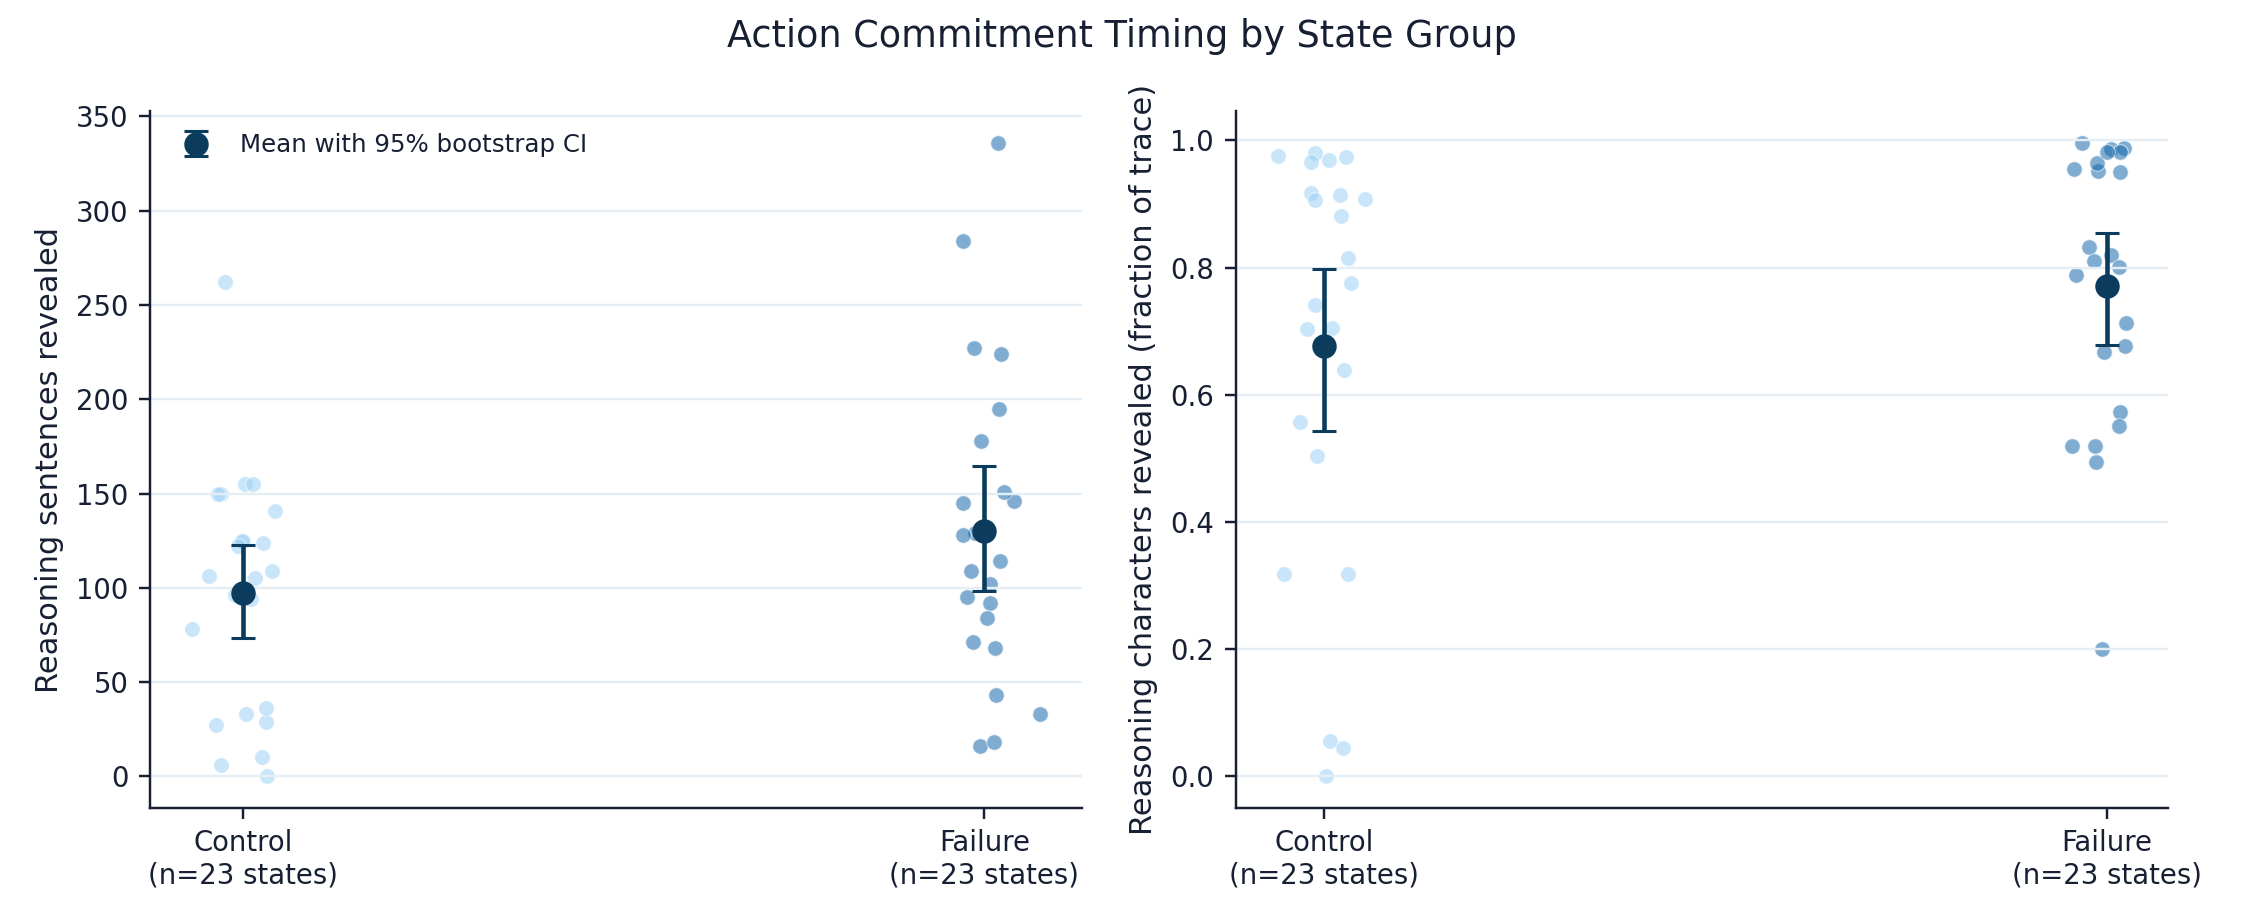
\includegraphics[width=\columnwidth]{figures/commitment_timing_matched46.png}
\caption{Commitment timing in 46 matched decisions. The left panel reports the
sentence index at commitment; the right reports the fraction of reasoning
characters revealed. Points are decisions. Large markers are group means and
bars are 95\% intervals obtained by resampling decisions within each group.}
\label{fig:commitment-timing-matched46}
\end{figure}

\paragraph{Belief-clause sufficiency control.}
For 46 decisions from 31 trajectories, we remove the chain of thought while
retaining the grid and key status, then add one fixed block of clauses. Actions
are obtained from candidate-token probabilities at temperature $0.7$.

\begin{table}[htbp]
\centering
\small
\begin{tabular}{lrrr}
\toprule
Condition & Different & Mean TV & Optimal \\
\midrule
Full CoT & 0/46 & 0.000 & 38/46 \\
Grid only & 34/46 & 0.723 & 17/46 \\
Model reports & 31/46 & 0.677 & 23/46 \\
Verified facts & 36/46 & 0.767 & 11/46 \\
One false wall fact & 36/46 & 0.750 & 20/46 \\
Irrelevant clauses & 31/46 & 0.686 & 22/46 \\
\bottomrule
\end{tabular}
\caption{Action readouts after replacing the chain of thought with state-belief
clauses. ``Different'' counts decisions whose top action differs from the
full-chain action. TV is total variation distance from the full-chain action
distribution. Verified facts are simulator-derived; the false condition flips
one wall fact.}
\label{tab:belief-clause-sufficiency}
\end{table}

The model-report and irrelevant-clause conditions differ little in optimal
rate, while verified facts perform worse than either. The six local facts are
therefore not a sufficient replacement for the chain of thought. The
irrelevant-clause result also shows that wording and clause order remain
confounds.

\paragraph{Offline action-distribution change points.}
A trend-only BEAST analysis detects 160 change points across 44 of 46 decisions.
Of these, 86.9\% lie within three sentences of a recommendation change, compared
with 65.3\% for progress-matched control sentences (randomisation
$p=0.0005$). Proximity is also above the matched rate for optimality losses
(33.1\% versus 26.2\%, $p=0.0060$) and recoveries (41.9\% versus 29.4\%,
$p=0.0005$). Detection uses the complete action-probability series, so these
are retrospective candidate boundaries rather than online predictions or
causal events.

\paragraph{Semantic labels at change points.}
We compare 160 detected change-point sentences with 160 blinded, same-decision
controls matched on reasoning progress and sentence length. The primary test
uses the 152 pairs within $0.10$ reasoning progress. The four-way semantic
distributions do not differ reliably (paired permutation $p=0.219$). Route
deliberation is 5.3 percentage points more frequent at change points, but its
95\% interval obtained by resampling complete trajectories,
$[-2.1,12.0]$, includes zero. These
results do not support a single verbal operation underlying action changes.

\paragraph{Activation event classification.}
Across 7,038 sentence positions from 46 decisions, layer-15 sentence-mean
activations are associated with contemporaneous action-change labels (linear
CKA $0.00437$, permutation-null mean $0.00062$, $p=0.005$). Adding belief
and activation features to a behavioural baseline improves action-change
AUROC by $0.030$ and log loss by $0.0085$ on complete trajectories excluded
from fitting. For
optimal-to-suboptimal transitions, however, the best added signal is the belief
panel and it does not improve held-out performance (AUROC change $-0.011$,
log-loss improvement $-0.0009$). Association at an event is therefore not
evidence of advance prediction or causal use.

\section{Semantic and Clustering Analyses}\label{app:semantic-clustering}
\subsection{Judge-generated Semantic Labels}
\label{app:judge_semantic_labels}

\paragraph{Data and annotation.}
This analysis covers 7,038 sentences from 46 matched decisions in 31
trajectories. It uses different data and labels from the four-class analysis of
141,377 sentences from 1,004 decisions in \Cref{sec:reasoning}; the 20,366
sentences used to interpret the activation clusters are a subset of that larger
analysis. The present data come from the same matched cohort as the
reasoning-time action, belief, and activation analyses, although their exact
rows differ after alignment and filtering.

A \texttt{gpt-oss-20b} judge receives the preceding reasoning
and target sentence, with later reasoning and experimental measurements hidden.
It may assign more than one of nine functions: state readout, route planning,
verification, correction, new inference, consolidation, restatement,
procedural continuation, and action commitment. We ran the same prompt twice
independently. Both runs produced valid labels for 7,036 sentences. Exact label
sets agree on 74.9\% of sentences, with an interval of
$[73.8\%,75.9\%]$ from resampling complete trajectories. Derived primary
labels agree on 85.4\% with an interval of $[84.4\%,86.5\%]$ and Cohen's
$\kappa=0.820$. These values measure annotation
repeatability, not agreement with human labels.

\begin{table}[htbp]
\centering
\small
\begin{tabular}{lrr}
\toprule
Function & Run 1 rate & Between-run Dice \\
\midrule
State readout & 36.9\% & 0.923 \\
Route planning & 21.4\% & 0.918 \\
Verification & 21.5\% & 0.823 \\
Correction & 0.4\% & 0.632 \\
New inference & 39.7\% & 0.872 \\
Consolidation & 1.4\% & 0.558 \\
Restatement & 11.5\% & 0.777 \\
Procedural continuation & 5.1\% & 0.915 \\
Action commitment & 5.6\% & 0.934 \\
\bottomrule
\end{tabular}
\caption{Frequency and repeatability of the matched-cohort semantic labels.
Rates need not sum to 100\% because labels may overlap. Dice measures agreement
on the positive examples for each label across two independent runs.}
\label{tab:semantic-label-repeatability}
\end{table}

\paragraph{Temporal structure and prediction.}
The labels occur in a reproducible order. Relative to labels shuffled within
each trajectory and reasoning-progress bin, adjacent primary labels contain
0.118 and 0.120 additional bits of mutual information in the two runs
($p=0.0002$ for each). Twelve
label-to-label transitions and 27 three-sentence sequences are enriched after
false-discovery-rate correction in both runs. However, adding the current
semantic labels to action probabilities, action entropy, reasoning progress,
regime duration, and regime history does not improve prediction of later
regime changes in any of 28 corrected horizon tests. The labels describe
recurring reasoning sequences but do not provide an additional action-change
monitor in this dataset.



\subsection{Reasoning-Step Clustering Details}
\label{app:reasoning-clustering}

This appendix provides additional details on the sentence-level activation
clustering used in \Cref{app:semantic-clustering}. The main analysis uses
sentence-mean representations from layer 15 of \texttt{gpt-oss-20b}. For
each reasoning sentence, we mean-pool the token-level hidden states over the
sentence span to obtain one 2,880-dimensional vector. We randomly sample
25,000 of the 153,622 sentence representations, reduce them to 100 principal
components retaining 77.84\% of the activation variance, and
$\ell_2$-normalise the resulting vectors before clustering.

\paragraph{Clustering method comparison.}
We compare MiniBatch K-means, HDBSCAN, and Gaussian mixture models using both
sentence-mean and sentence-final representations. Sentence-mean HDBSCAN
achieves the highest silhouette coefficient and lowest intra-cluster
dispersion, but assigns 77.1\% of sentences to noise. Sentence-mean K-means
provides a complete partition of the data and achieves the highest
inter-cluster dispersion and Calinski--Harabasz score among the
complete-coverage methods. We therefore use sentence-mean K-means for the
main analysis, while treating HDBSCAN as a secondary method for identifying
high-density motifs.

The repository does not record a prespecified selection rule for $K=12$, so all cluster results are treated as exploratory.

\begin{table}[htbp]
\centering
\small
\begin{tabular}{lccccc}
\toprule
Method & Silhouette & Inter-disp. & Intra-disp. & CH & Noise \\
\midrule
Mean K-means     & 0.138 & 905.0 & 0.600 & 1509.0 & 0.0\% \\
Mean HDBSCAN     & 0.431 & 263.9 & 0.225 & 1172.9 & 77.1\% \\
Mean GMM         & 0.075 & 755.6 & 0.666 & 1135.3 & 0.0\% \\
Final K-means    & 0.128 & 782.6 & 0.655 & 1194.0 & 0.0\% \\
Final HDBSCAN    & 0.381 & 297.2 & 0.293 & 1014.0 & 64.8\% \\
Final GMM        & 0.074 & 641.3 & 0.718 & 893.7 & 0.0\% \\
\bottomrule
\end{tabular}
\caption{Clustering quality for sentence-mean and sentence-final hidden
representations. Inter-dispersion and intra-dispersion measure separation
between clusters and compactness within clusters, respectively. CH denotes
the Calinski--Harabasz score.}
\label{tab:reasoning-clustering}
\end{table}

\begin{figure}[htbp]
    \centering

    \begin{subfigure}[t]{0.49\textwidth}
        \centering
        \includegraphics[width=\linewidth]{figures/hdbscan_mean.png}
        \caption{HDBSCAN}
        \label{fig:hdbscan-clusters}
    \end{subfigure}
    \hfill
    \begin{subfigure}[t]{0.49\textwidth}
        \centering
        \includegraphics[width=\linewidth]{figures/k_means_mean.png}
        \caption{MiniBatch K-means}
        \label{fig:kmeans-clusters}
    \end{subfigure}

    \caption{
    Two-dimensional PCA visualisation of sentence-level hidden
    representations. HDBSCAN identifies a smaller number of dense regions
    while assigning many points to noise, whereas K-means provides a complete
    partition of the representation space.
    }
    \label{fig:clustering-comparison}
\end{figure}

\paragraph{Cluster interpretation.}
The clustering procedure is unsupervised and does not use semantic labels.
For interpretation only, we inspect representative sentences from each
cluster and compare cluster assignments with independently assigned semantic
reasoning annotations. We then attach short descriptive names to the numeric
cluster IDs. These names are post-hoc summaries and are not used during
clustering.

Among 20,366 sentences with exact alignment to the semantic annotations,
K-means reaches normalised mutual information of 0.131. Thus, the activation
clusters capture structure that is related to, but not identical with, the
semantic categories. HDBSCAN yields higher semantic purity on its non-noise
subset, with normalised mutual information of 0.297 and homogeneity of
0.473, but leaves approximately 80\% of downstream sentences unassigned.

\begin{table}[htbp]
\centering
\small
\begin{tabular}{lll}
\toprule
Cluster & Descriptive interpretation & Example reasoning role \\
\midrule
\(C_0\)  & Path initiation & Beginning or extending a route \\
\(C_1\)  & Local world-state checking & Reading nearby grid structure \\
\(C_2\)  & Route execution & Following a selected path \\
\(C_3\)  & Door-mechanics reasoning & Reasoning about key or door state \\
\(C_4\)  & Alternative-route exploration & Considering another route \\
\(C_5\)  & Grid-state setup & Reconstructing the current state \\
\(C_6\)  & Detailed state readout & Explicitly checking environment details \\
\(C_7\)  & Route consolidation & Consolidating a planned path \\
\(C_8\)  & Blockage verification & Checking whether a movement is blocked \\
\(C_9\)  & Local route tracing & Tracing immediate movement options \\
\(C_{10}\) & Decision revision & Revising or transitioning between choices \\
\(C_{11}\) & Action conclusion & Expressing or consolidating the final action \\
\bottomrule
\end{tabular}
\caption{Post-hoc descriptive interpretations of the K-means clusters.
Cluster IDs are used throughout the quantitative analysis; the descriptions
are provided only to aid interpretation.}
\label{tab:cluster-labels}
\end{table}

The descriptive names are not used as quantitative labels.

The coarse semantic comparison is consistent with several of these
descriptions. Clusters \(C_6\), \(C_5\), and \(C_1\) contain a larger
proportion of world-reading sentences, whereas \(C_2\), \(C_7\), and \(C_4\)
contain more solving-oriented sentences. \(C_{11}\) contains a larger
answering component. A finer multi-label analysis also shows enrichment for
specific reasoning functions: \(C_2\) is enriched approximately
\(9.8\times\) for action commitment, \(C_{10}\) \(10.1\times\) for
correction, \(C_8\) \(2.8\times\) for verification, and \(C_0\)
\(5.6\times\) for procedural continuation.

\paragraph{Cluster frequencies around commitment.}
The distribution of clusters changes across the commitment point. After
commitment, \(C_{11}\), \(C_2\), and \(C_7\) increase in frequency by
12.8, 6.3, and 5.6 percentage points, respectively. In contrast, \(C_5\),
\(C_6\), \(C_0\), and \(C_1\) decrease by 9.8, 7.4, 4.4, and 2.7 percentage
points. This pattern is consistent with a transition from state
interpretation and revision toward route execution and explicit action
conclusion.

To control for the fact that commitment tends to occur at particular
positions in the reasoning trace, we compare true commitment sentences with
position-matched control sentences drawn from the same decisions. The largest
difference is observed for \(C_{10}\), which occurs in 14.0\% of true
commitment sentences compared with 5.9\% under the matched control. Smaller
excesses are observed for \(C_9\) and \(C_2\).

\begin{table}[htbp]
\centering
\small
\begin{tabular}{lrrr}
\toprule
Cluster & True commitment & Matched control & Excess \\
\midrule
\(C_{10}\) & 14.0\% & 5.9\% & \(+8.2\) pp \\
\(C_9\)    & 11.6\% & 8.4\% & \(+3.2\) pp \\
\(C_2\)    & 9.3\% & 6.8\% & \(+2.5\) pp \\
\(C_5\)    & 15.1\% & 13.5\% & \(+1.6\) pp \\
\(C_7\)    & 5.5\% & 4.5\% & \(+1.0\) pp \\
\bottomrule
\end{tabular}
\caption{Frequency of selected K-means clusters at true commitment positions
and at position-matched control positions from the same decisions.}
\label{tab:commitment-clusters-app}
\end{table}

This comparison is descriptive because no uncertainty estimate was retained for these five cluster differences.

\paragraph{Clusters at action-revision events.}
We also test whether particular activation-defined reasoning states are
associated with changes in the currently preferred action. Approximately
4.59\% of reasoning sentences contain at least one such change. Relative to
a within-decision shuffled-event control, \(C_6\), \(C_{10}\), \(C_9\), and
\(C_5\) are enriched at action-preference changes by factors of
\(1.65\times\), \(1.64\times\), \(1.41\times\), and \(1.33\times\),
respectively. All four effects remain significant after false-discovery-rate
correction (\(q=0.0024\)).

The same clusters occur around both losses and recoveries of action
optimality. For optimal-to-suboptimal transitions, enrichment factors are
\(2.07\times\), \(1.48\times\), \(1.45\times\), and \(1.26\times\) for
\(C_6\), \(C_{10}\), \(C_9\), and \(C_5\), respectively. For
suboptimal-to-optimal transitions, the corresponding factors are
\(1.77\times\), \(1.59\times\), \(1.44\times\), and \(1.35\times\).
Because the same clusters are associated with both directions of change, we
interpret them as reasoning states associated with decision revision rather
than as error-specific states.

\begin{table}[htbp]
\centering
\small
\begin{tabular}{lccc}
\toprule
Cluster & Action change & Accuracy drop & Accuracy recovery \\
\midrule
\(C_6\)    & \(1.65\times\) & \(2.07\times\) & \(1.77\times\) \\
\(C_{10}\) & \(1.64\times\) & \(1.48\times\) & \(1.59\times\) \\
\(C_9\)    & \(1.41\times\) & \(1.45\times\) & \(1.44\times\) \\
\(C_5\)    & \(1.33\times\) & \(1.26\times\) & \(1.35\times\) \\
\bottomrule
\end{tabular}
\caption{Enrichment of sentence-level activation clusters at
action-preference changes and changes in action optimality, relative to
within-decision shuffled-event controls.}
\label{tab:reasoning-events-app}
\end{table}

The immediately preceding sentence shows a similar pattern. For example,
\(C_5\) is enriched \(2.09\times\) before an optimal-to-suboptimal transition
and \(2.47\times\) before a suboptimal-to-optimal transition.

\paragraph{Exploratory cluster sequences.}
Finally, we examine whether short transitions between activation clusters are
overrepresented near commitment. Examples include
\(C_8\!\rightarrow C_{10}\) (\(4.75\times\)),
\(C_{10}\!\rightarrow C_{10}\) (\(2.87\times\)), and
\(C_7\!\rightarrow C_{10}\) (\(2.71\times\)). Enriched three-step sequences
include \(C_6\!\rightarrow C_5\!\rightarrow C_5\) (\(3.26\times\)) and
\(C_{10}\!\rightarrow C_{10}\!\rightarrow C_{10}\) (\(3.86\times\)).
Because the number of possible sequences is large and these analyses are
exploratory, we do not use them to support the main conclusions.
\section{Intervention Details and Robustness}\label{app:intervention-robustness}
\paragraph{Whole-chain replacement.}
We pair the prompt of decision $A$ with a prefix from decision $B$, whose emitted action differs, cutting at about 10, 50, or 90\% of $B$'s reasoning. There are 396 mismatched pairs and 396 congruent controls, each evaluated in an independent forward pass. In mismatched pairs, probability assigned to $a_B$ ranges from 0.598 to 0.673, compared with 0.129 to 0.165 for $a_A$. The forced top action equals $a_B$ in 61.4, 66.7, and 68.9\% of early, middle, and late cuts.
\begin{figure}[t]
\centering
\includegraphics[width=0.62\textwidth]{figures/mismatched_prompt_cot_tracking.png}
\caption{Whole-chain replacement. A prompt from decision $A$ is paired with reasoning from decision $B$. The forced action follows the foreign reasoning more than the visible state.}\label{fig:cot-swap}
\end{figure}

\paragraph{Activation controls and scope.}
Steering edits use a fixed 512-dimensional projection at layers 10, 15, and 18, with magnitudes up to the residual-state norm. Random controls have the same norm. Transplants are tested at layers 3, 10, 15, and 18. Rank-1 and rank-3 replacements produce no targeted flips; the full-window overwrite reaches 20.8\% at its best layer. Removing an attention or MLP sub-block changes up to 29.2\% of answers but has no intended target and is therefore a damage test. Appending an instruction that disavows mismatched reasoning recovers 0.14\% of the lost action probability. No known positive-control steering direction was available. These experiments concern the final reasoning-window tokens and do not test pre-reasoning activation edits.

%%%%%%%%%%%%%%%%%%%%%%%%%%%%%%%%%%%%%%%%%%%%%%%%%%%%%%%%%%%%

\newpage
\input{checklist.tex}


\end{document}